\chapter{CGRA-based accelerator}
\label{chapter:cgra}

In this chapter, the fundamentals about Coarse Grained Reconfigurable Arrays
(CGRAs) and why they can be used for accelerating CNNs are briefly
explained. The Deep Versat CGRA architecture, which will be used in this work
for accelerating the YOLOv3 detector, is described. The chapter ends with a
basic example of the implementation of a 2D convolution using a single layer of
the Deep Versat core.

\section{CGRA architecture}
\label{section:cgra_arch}

A CGRA is a collection of programmable functional units (FUs) and embedded memories interconnected by programmable switches~\cite{lopes:versat}. The interconnections are reconfigurable at run-time, which allows to form different hardware datapaths to accelerate distinct computations for the same application. CGRAs are reconfigurable at the word-level and the hardware units can be programmed in any execution cycle.

Typically, CGRAs consist of a reconfigurable array, which is mainly used to accelerate program loops, and a conventional CPU, which executes the non-loop code of a given application and controls the configuration of the array. Thus, CGRAs can be used as hardware co-processors to accelerate parts of the algorithms that are slow or energy inefficient in regular CPUs~\cite{valter:deep_versat}.  

The FPGA-based architecture for accelerating CNNs proposed on previous works, which was studied in section \ref{subsection:acc_opt}, is the same as the CGRA architecture. Both consist of a spatial array of processing elements (i.e., functional units) with data flowing through an interconnection network and memory is located as close as possible to the computational units~\cite{auto_tuning_cgra}. 

The reconfigurable array is suitable for accelerating program loops, which fits with the implementation of the convolutional layers. For all these reasons, a CGRA-based architecture can be used for accelerating CNNs. For instance,~\cite{alexnet_cgra} implemented the AlexNet network in a CGRA by using 16 PEs and 9 parallel multipliers with fixed-point arithmetic of 8 bits for the image pixels, 16 bits for the weights, bias and output feature maps and 32 bits for intermediate results, achieving a throughput of 141 GOPs, which is comparable with the ones obtained in Table~\ref{tab:comp_fpga_acc}. An auto-tuning compiler to map CNNs in CGRA architectures by exploring loop optimization techniques is proposed in~\cite{auto_tuning_cgra} . The author claims that the developed CGRA outperforms, in terms of energy per inference, other ARM-based accelerators.

\section{Deep Versat}
\label{section:versat}

Versat \cite{lopes:versat} is a 32-bit CGRA architecture developed at the INESC-ID Research Institute capable of being configured on the fly, without using pre-compiled configurations, through partial reconfiguration. The ability of generating configuration sequences from stored routines, instead of storing the configuration itself, allows to exploit the similarity between configurations as only distinct bits need to be changed, which results in a faster and less energy consuming configuration. 

Versat is composed of FUs organized in a full mesh topology, which limits the number of FUs that an application could use, due to the increase of the circuit delay caused by the selection multiplexers. To overcome this limitation, a multi-layer architecture composed of a set of Versats, called Deep Versat, was proposed in a master thesis~\cite{valter:deep_versat}. With more layers, programs can use more FUs. Layers are stacked in a ring structure, as shown in Fig.~\ref{fig:deep_versat}, to limit the number of connections and prevent a frequency drop.

\vspace{-0.3cm}
\begin{figure}[!htb]
  \centering
  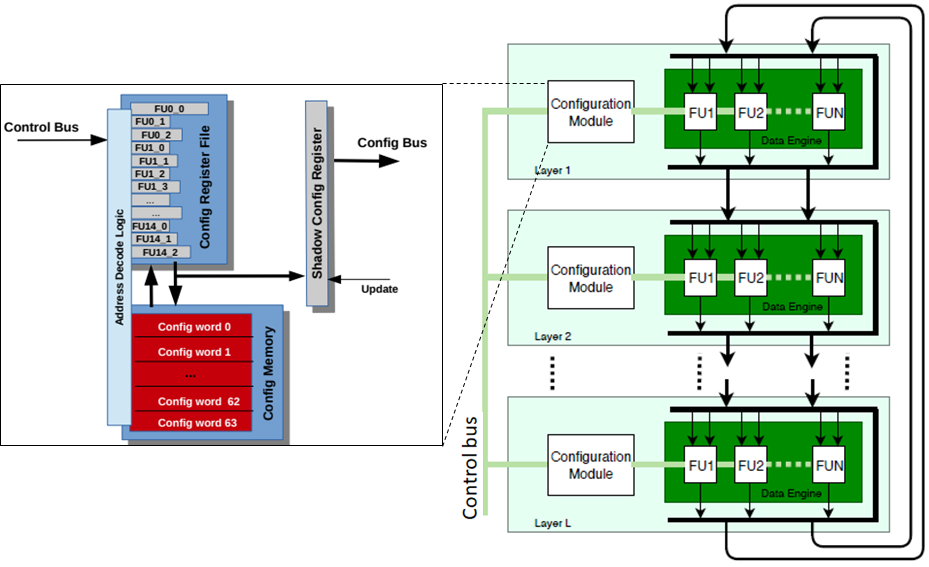
\includegraphics[width=0.85\textwidth]{Figures/deep_versat.png}
  \caption{Deep Versat architecture (adapted from~\cite{valter:deep_versat}).}
  \label{fig:deep_versat}
\end{figure}
\vspace{-0.15cm}

%FIX é Control Bus (do picorv) na figura e não Config Bus. Nota que não serve apenas para
%config mas tb para dar o start e ver se acabou. Do lado esquerdo da figura está
%certo e diz Control bus. Config. bus é o que liga o CM ao DE --> (DONE)

Each Versat has a data engine and a configuration module. In the data engine,
the FUs are interconnected by a data bus which concatenates the 32-bit output of
each FU of the current and of the previous layer (memories have two 32-bit
outputs as they are dual-port). As the interconnection follows a full mesh
topology, each FU can select any section from the data bus by means of a
programmable multiplexer, depending on the configuration defined in the
configuration bus.

The configuration module is composed by (1) the Configuration Shadow Register,
which stores the configuration currently being executed by the respective data
engine, (2) the Configuration Register File, which holds the next configuration,
and (3) the Configuration Memory, which saves frequently used configurations. The configuration bus connects the data engine and the configuration
module.

Currently, the functional units available include dual-port memories, arithmetic
logic units (ALUs), multipliers, multiplier and accumulators (called MulAdd) and
barrel shifters. The number of FUs is configured at compile time. Each FU holds
different configuration parameters based on their functionality: \\

\vspace{-0.4cm} \textbf{Dual-port memory}: Besides the 2 input and output ports,
each Versat memory has two Address Generation Units (AGUs) which consist in two
cascaded counters that allow for the execution of two nested loops in one
configuration. The AGU can be programmed to generate the address sequence for
accessing data from the memory during the execution of a program loop or to
generate a counter to control, for example, a MulAdd. The parameters are
described in Table~\ref{tab:versat_agu_param}.

%FIX below note that the base addresses are not parameters of the FU but of the
%system. The FU itself does not store its base address. Only the system needs to
%know it to be able to access it. However in the software API it makes sense to
%associate each FU base address with the FU class. --> (DONE)

\begin{table}[!htb]
    \footnotesize
    \centering
    \caption{Parameters of the dual-port memories.}
    \label{tab:versat_agu_param}
    \begin{tabular}{|c|c|c|c|}
    \hline
    Parameter   &  Description                          & Parameter     &  Description                                      \\ \hline
    start       & Memory start address                  & per           & N.º of inner loop iterations (period)             \\ \hline
    iter        & N.º of outer loop iterations          & duty          & N.º of cycles in a period where memory is enabled \\ \hline
    incr        & Increment of the inner loop           & sel           & Address of the input FU                           \\ \hline
    delay       & N.º of clock cycles before AGU starts & shift         & Additional increment at the end of each period    \\ \hline
    ext         & Flag for bypassing the AGU            & \multicolumn{2}{c|}{}                                                   \\ \hline
    \end{tabular}
\end{table}

%The nested loops computation and respective parameters of the AGU are represented in Fig. \ref{fig:agu_nested_loops}. 

%\begin{figure}[!htb]
%  \centering
%  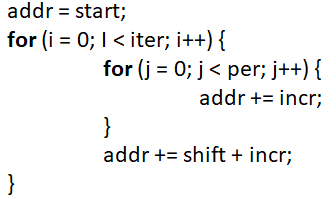
\includegraphics[width=0.3\textwidth]{Figures/versat_agu.png}
%  \caption{AGU nested loops computation.}
%  \label{fig:agu_nested_loops}
%\end{figure} 

\textbf{ALU / Multiplier}: These FUs have 3 parameters: the two input operand addresses and the type of operation. In the case of the ALU,
the most common operations include logic operations (e.g. AND, OR) and
additions. The multiplier has a latency of three clock cycles and allows to
choose the upper or lower 32-bit part of the 64-bit multiplication result.\\

\vspace{-0.4cm} \textbf{Barrel shifter}: The barrel shifter has a latency of 1 clock cycle and has 3 parameters: the address of the operand to be shifted, the size of the shift and the type/direction of the shift (e.g, right/left, logic/arithmetic).\\

\vspace{-0.4cm} \textbf{MulAdd}: The MulAdd was also added by~\cite{valter:deep_versat}. This FU has 4 configuration parameters: the two operand addresses, the reset and the type of operation. The reset controls how many accumulations to perform and can be applied with a counter from a memory AGU.  

%FIX the counter is not a parameter in the hw (is it in the sw?). The FU has an
%input to control when it resets. -> DONE

\subsection{System integration}

As previously mentioned, a CGRA is typically accompanied by a CPU. As shown in Fig.~\ref{fig:deep_versat_system}, Deep Versat is controlled by a RISC-V soft-processor. In this system, the processor accesses peripherals through its memory bus. Deep Versat can be seen as two peripherals, one for the control bus to start its execution and manipulate the configuration registers and another one for the data bus, which is used for data transfers. The UART module is another peripheral mainly used for debugging.

\begin{figure}[!htb]
  \centering
  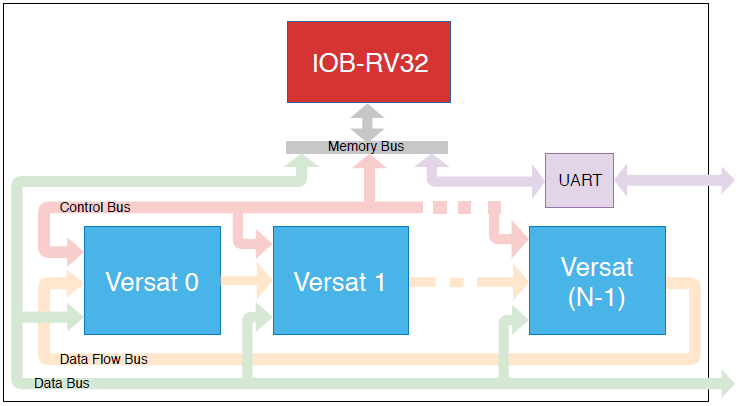
\includegraphics[width=0.6\textwidth]{Figures/deep_versat_system.png}
  \caption{Deep Versat system~(\cite{valter:deep_versat}).}
  \label{fig:deep_versat_system}
\end{figure}

%\vspace{-0.5cm}
\subsection{Basic implementation}

The RISC-V processor is programmed with a standard GNU toolchain, which contains compilers for C and C++. Therefore, Deep Versat also includes an API in C++ to enhance its configuration process. To show the usage of this API, a simple 2D convolution, using a single Versat layer, between a 5x5 feature map and a 3x3 kernel (without zero-padding) is exemplified in Fig.~\ref{fig:convolution_versat}. 

The feature map and the kernel are stored in different memories (mem0 and mem1). To read a 3x3 block from the feature map, a correct manipulation of the parameters in Table~\ref{tab:versat_agu_param} is needed. The parameters $iter$, $per$ and $duty$ are set to 3 in order to read one pixel per clock cycle across the 3 columns and 3 lines. The shift must be 2 to read the next row as data is stored in row-major order. For the kernel, 9 consecutive positions from mem1 are read. The second port (B) of this memory is used to generate a counter from 0 to 8 to control the number of accumulations in the MulAdd, whose inputs are connected to both memories. The results are stored in another memory (mem2). Finally, the loops for iterating through the feature map are defined in software to configure the start address of the read memories and to run the Versat at each iteration. 

\vspace{+0.1cm}

\begin{figure}[!htb]
  \centering
  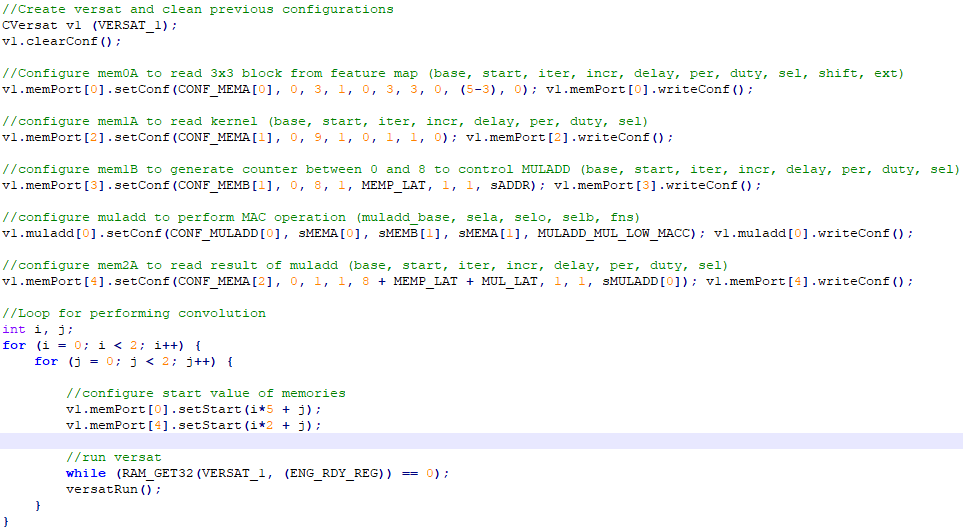
\includegraphics[width=\textwidth]{Figures/versat_convolution.png}
  \caption{Example of 2D convolution with one Versat.}
  \label{fig:convolution_versat}
\end{figure}
\vspace{-0.4cm}

\subsubsection{Final remarks}

This simple example showed how to accelerate loops using a single Versat layer. By using more layers from the Deep Versat architecture and by applying loop optimization techniques, convolutional layers from complex CNNs such as the YOLOv3 detector can be accelerated. In the next chapter, the proposed methodology and the expected planning of this work are described.
